% 2-15-rb-tree.tex

%%%%%%%%%%%%%%%%%%%%
\documentclass[a4paper, justified]{tufte-handout}

% hw-preamble.tex

% geometry for A4 paper
% See https://tex.stackexchange.com/a/119912/23098
\geometry{
  left=20.0mm,
  top=20.0mm,
  bottom=20.0mm,
  textwidth=130mm, % main text block
  marginparsep=5.0mm, % gutter between main text block and margin notes
  marginparwidth=50.0mm % width of margin notes
}

% for colors
\usepackage{xcolor} % usage: \color{red}{text}
% predefined colors
\newcommand{\red}[1]{\textcolor{red}{#1}} % usage: \red{text}
\newcommand{\blue}[1]{\textcolor{blue}{#1}}
\newcommand{\teal}[1]{\textcolor{teal}{#1}}

\usepackage{todonotes}

% heading
\usepackage{sectsty}
\setcounter{secnumdepth}{2}
\allsectionsfont{\centering\huge\rmfamily}

% for Chinese
\usepackage{xeCJK}
\usepackage{zhnumber}
\setCJKmainfont[BoldFont=FandolSong-Bold.otf]{FandolSong-Regular.otf}

% for fonts
\usepackage{fontspec}
\newcommand{\song}{\CJKfamily{song}} 
\newcommand{\kai}{\CJKfamily{kai}} 

% To fix the ``MakeTextLowerCase'' bug:
% See https://github.com/Tufte-LaTeX/tufte-latex/issues/64#issuecomment-78572017
% Set up the spacing using fontspec features
\renewcommand\allcapsspacing[1]{{\addfontfeature{LetterSpace=15}#1}}
\renewcommand\smallcapsspacing[1]{{\addfontfeature{LetterSpace=10}#1}}

% for url
\usepackage{hyperref}
\hypersetup{colorlinks = true, 
  linkcolor = teal,
  urlcolor  = teal,
  citecolor = blue,
  anchorcolor = blue}

\newcommand{\me}[4]{
    \author{
      {\bfseries 姓名:}\underline{#1}\hspace{2em}
      {\bfseries 学号:}\underline{#2}\hspace{2em}\\[10pt]
      {\bfseries 评分:}\underline{#3\hspace{3em}}\hspace{2em}
      {\bfseries 评阅:}\underline{#4\hspace{3em}}
  }
}

% Please ALWAYS Keep This.
\newcommand{\noplagiarism}{
  \begin{center}
    \fbox{\begin{tabular}{@{}c@{}}
      请独立完成作业,不得抄袭。\\
      若得到他人帮助, 请致谢。\\
      若参考了其它资料,请给出引用。\\
      鼓励讨论,但需独立书写解题过程。
    \end{tabular}}
  \end{center}
}

\newcommand{\goal}[1]{
  \begin{center}{\fcolorbox{blue}{yellow!60}{\parbox{0.50\textwidth}{\large 
    \begin{itemize}
      \item 体会``思维的乐趣''
      \item 初步了解递归与数学归纳法 
      \item 初步接触算法概念与问题下界概念
    \end{itemize}}}}
  \end{center}
}

% Each hw consists of four parts:
\newcommand{\beginrequired}{\hspace{5em}\section{作业 (必做部分)}}
\newcommand{\beginoptional}{\section{作业 (选做部分)}}
\newcommand{\beginot}{\section{Open Topics}}
\newcommand{\begincorrection}{\section{订正}}
\newcommand{\beginfb}{\section{反馈}}

% for math
\usepackage{amsmath, mathtools, amsfonts, amssymb}
\newcommand{\set}[1]{\{#1\}}

% define theorem-like environments
\usepackage[amsmath, thmmarks]{ntheorem}

\theoremstyle{break}
\theorempreskip{2.0\topsep}
\theorembodyfont{\song}
\theoremseparator{}
\newtheorem{problem}{题目}[subsection]
\renewcommand{\theproblem}{\arabic{problem}}
\newtheorem{ot}{Open Topics}

\theorempreskip{3.0\topsep}
\theoremheaderfont{\kai\bfseries}
\theoremseparator{:}
\theorempostwork{\bigskip\hrule}
\newtheorem*{solution}{解答}
\theorempostwork{\bigskip\hrule}
\newtheorem*{revision}{订正}

\theoremstyle{plain}
\newtheorem*{cause}{错因分析}
\newtheorem*{remark}{注}

\theoremstyle{break}
\theorempostwork{\bigskip\hrule}
\theoremsymbol{\ensuremath{\Box}}
\newtheorem*{proof}{证明}

% \newcommand{\ot}{\blue{\bf [OT]}}

% for figs
\renewcommand\figurename{图}
\renewcommand\tablename{表}

% for fig without caption: #1: width/size; #2: fig file
\newcommand{\fig}[2]{
  \begin{figure}[htbp]
    \centering
    \includegraphics[#1]{#2}
  \end{figure}
}
% for fig with caption: #1: width/size; #2: fig file; #3: caption
\newcommand{\figcap}[3]{
  \begin{figure}[htbp]
    \centering
    \includegraphics[#1]{#2}
    \caption{#3}
  \end{figure}
}
% for fig with both caption and label: #1: width/size; #2: fig file; #3: caption; #4: label
\newcommand{\figcaplbl}[4]{
  \begin{figure}[htbp]
    \centering
    \includegraphics[#1]{#2}
    \caption{#3}
    \label{#4}
  \end{figure}
}
% for margin fig without caption: #1: width/size; #2: fig file
\newcommand{\mfig}[2]{
  \begin{marginfigure}
    \centering
    \includegraphics[#1]{#2}
  \end{marginfigure}
}
% for margin fig with caption: #1: width/size; #2: fig file; #3: caption
\newcommand{\mfigcap}[3]{
  \begin{marginfigure}
    \centering
    \includegraphics[#1]{#2}
    \caption{#3}
  \end{marginfigure}
}

\usepackage{fancyvrb}

% for algorithms
\usepackage[]{algorithm}
\usepackage[]{algpseudocode} % noend
% See [Adjust the indentation whithin the algorithmicx-package when a line is broken](https://tex.stackexchange.com/a/68540/23098)
\newcommand{\algparbox}[1]{\parbox[t]{\dimexpr\linewidth-\algorithmicindent}{#1\strut}}
\newcommand{\hStatex}[0]{\vspace{5pt}}
\makeatletter
\newlength{\trianglerightwidth}
\settowidth{\trianglerightwidth}{$\triangleright$~}
\algnewcommand{\LineComment}[1]{\Statex \hskip\ALG@thistlm \(\triangleright\) #1}
\algnewcommand{\LineCommentCont}[1]{\Statex \hskip\ALG@thistlm%
  \parbox[t]{\dimexpr\linewidth-\ALG@thistlm}{\hangindent=\trianglerightwidth \hangafter=1 \strut$\triangleright$ #1\strut}}
\makeatother

% for footnote/marginnote
% see https://tex.stackexchange.com/a/133265/23098
\usepackage{tikz}
\newcommand{\circled}[1]{%
  \tikz[baseline=(char.base)]
  \node [draw, circle, inner sep = 0.5pt, font = \tiny, minimum size = 8pt] (char) {#1};
}
\renewcommand\thefootnote{\protect\circled{\arabic{footnote}}} % feel free to modify this file
%%%%%%%%%%%%%%%%%%%%
\title{第3-6讲: 树}
\me{林凡琪}{211240042}{}{}
\date{\zhtoday} % or like 2019年9月13日
%%%%%%%%%%%%%%%%%%%%
\begin{document}
\maketitle
%%%%%%%%%%%%%%%%%%%%
\noplagiarism % always keep this line
%%%%%%%%%%%%%%%%%%%%
\begin{abstract}
  % \begin{center}{\fcolorbox{blue}{yellow!60}{\parbox{0.65\textwidth}{\large 
  %   \begin{itemize}
  %     \item 
  %   \end{itemize}}}}
  % \end{center}
\end{abstract}
%%%%%%%%%%%%%%%%%%%%
\beginrequired

%%%%%%%%%%%%%%%
\begin{problem}[CZ 4.4]
Let $G$ be a connected graph and let $e1$ and $e2$ be two edges of $G$. Prove that $G − e1 − e2$ has three components if and only if both $e1$ and $e2$ are bridges in $G$.
\end{problem}

\begin{solution}
  若$e1$和$e2$为割边,$G-e1$为有两个连通分支$G1$和$G2$。假设边$e2$在连通分支$G1$中。在这个连通分支中将$e2$去掉,则该连通分支会新成两个连通分支$G3,G4$。此时即为$G-e1-e2$,共有$G2,G3,G4$三个连通分支。\\
  若$G-e1-e2$有三个连通分量,由于$G$连通,破坏连通性的方法为去掉割边,且去掉一条割边,只会多生成一个连通分支。因此,$e1,e2$必为割边。\\
  综上,得证。
\end{solution}
%%%%%%%%%%%%%%%

%%%%%%%%%%%%%%%
\begin{problem}[CZ 4.9]
Show that a graph of order n and size n − 1 need not be a tree.
\end{problem}

\begin{solution}
  \begin{figure}[htbp]
    \centering
    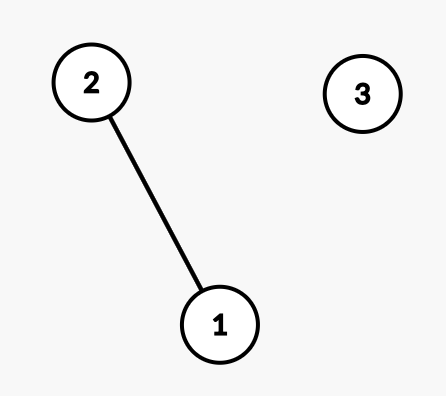
\includegraphics[width = 0.30\linewidth]{figs/a}
  \end{figure}

  n = 3
\end{solution}
%%%%%%%%%%%%%%%

%%%%%%%%%%%%%%%
\begin{problem}[CZ 4.14]
A certain tree $T$ of order $35$ is known to have $25$ vertices of degree $1$, two vertices of degree $2$, three vertices of degree $4$, one vertex of degree $5$ and two vertices of degree $6$. It also contains two vertices of the same (unknown) degree x. What is x?
\end{problem}

\begin{solution}
  由图论第一定理,25·1+2·2+3·4+1·5+2·6+2·x=2·34\\
  解得$x=5$
\end{solution}
%%%%%%%%%%%%%%%

%%%%%%%%%%%%%%%
\begin{problem}[CZ 4.22]
Let $T$ be a tree of order $n$. Show that the size of the complement of $\overline{T}$ is the same as the size of $K_{n − 1}$.
\end{problem}

\begin{solution}
  $K_{n-1}$的边数是$\frac{(n-1)(n-2)}{2}$\\
  $\overline{T}$的边数是$\frac{n(n-1)}{2}-(n-1)=\frac{(n-1)(n-2)}{2}$
\end{solution}
%%%%%%%%%%%%%%%

%%%%%%%%%%%%%%%
\begin{problem}[CZ 4.26]
Prove that an edge e of a connected graph is a bridge if and only if e belongs to every spanning tree of G.
\end{problem}

\begin{solution}
  充分:\\
  假设最后的生成树中不含这条割边,则根据定义,去掉这条割边后的图不连通。\\
  这与生成树的连通性矛盾。\\
  故生成树上一定有这条割边\\
  充分:\\
  若其不为割边,则可在其所在环上找一条边替代他,得到一个没有该边的生成树,故矛盾
\end{solution}
%%%%%%%%%%%%%%%

%%%%%%%%%%%%%%%
\begin{problem}[CZ 4.28]
\begin{figure}[htbp]
  \centering
  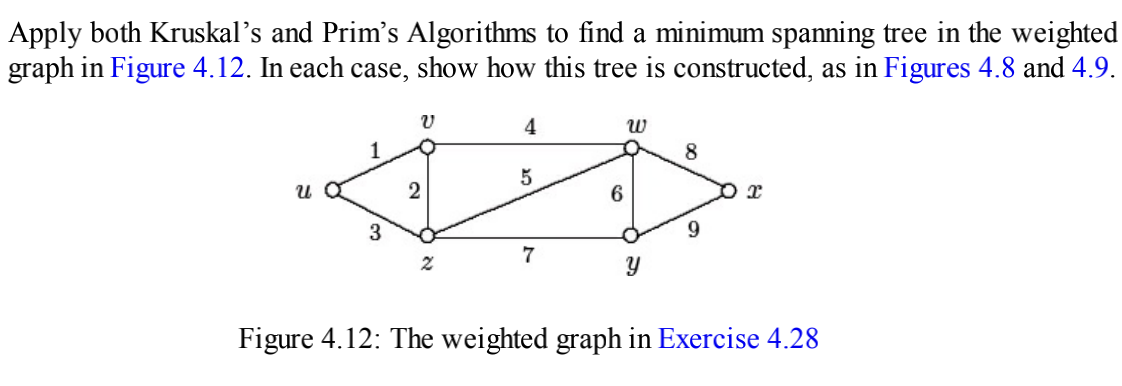
\includegraphics[width = 0.90\linewidth]{figs/b}
\end{figure}
\end{problem}

\begin{solution}
  Kruscal的加边顺序:$(u,v,1),(v,z,2),(v,w,4),(w,y,6),(w,x,8)$\\
  Kruscal的加边顺序(假设初使点为$u$):$(u,v,1),(v,z,2),(v,w,4),(w,y,6),(w,x,8)$\\
\end{solution}
%%%%%%%%%%%%%%%

%%%%%%%%%%%%%%%
\begin{problem}[CZ 4.30]
Let $G$ be a connected weighted graph and $T$ a minimum spanning tree of $G$. Show that $T$ is a unique minimum spanning tree of $G$ if and only if the weight of each edge e of $G$ that is not in $T$ exceeds the weight of every other edge on the cycle in $T + e$.
\end{problem}

\begin{solution}
  必要性:\\
  若$T$是唯一一棵最小生成树,则若$G$中不属于$T$的任一边$e$的权值都小于等于$T+e$的圈上某边的权值,则将该边去掉,加上边$e$,则可得到一棵权值相等或更小的生成树,与假设违背。故$G$中不属于$T$的任一边$e$的权值都大于$T+e$的圈上某边的权值\\
  充分性:\\
  若$G$中不属于$T$的任一边$e$的权值都大于$T+e$的圈上某边的权值,假设存在另一棵最小生成树$T1$,设$e=(u,v)\in T$且$e \notin T1$, 则在$T1$中$u\to v$的路径上,必存在一条边$e2$不在$T$中。由前提可知$e2$的权值大于$e$,显然将$e2$替换为$e$更优。故不存在$T2$,最小生成树唯一。
\end{solution}
%%%%%%%%%%%%%%%

%%%%%%%%%%%%%%%
\begin{problem}[CZ 4.36]
Find the number of spanning trees in the graph G\\
\begin{figure}[htbp]
  \centering
  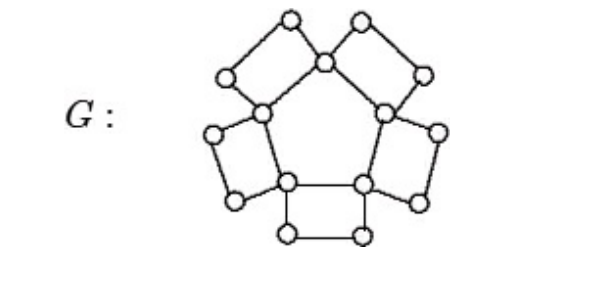
\includegraphics[width = 0.70\linewidth]{figs/aa}
\end{figure}
\end{problem}

\begin{solution}
  \begin{figure}[htbp]
    \centering
    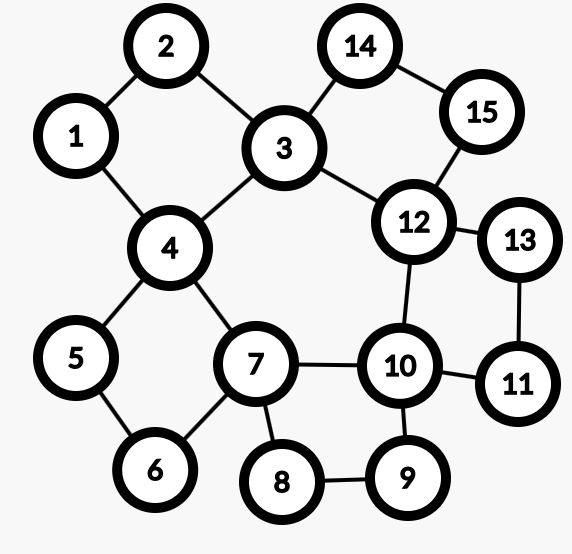
\includegraphics[width = 0.30\linewidth]{figs/g}
  \end{figure}

  先将其进行点标号。\\

  \begin{figure}[htbp]
    \centering
    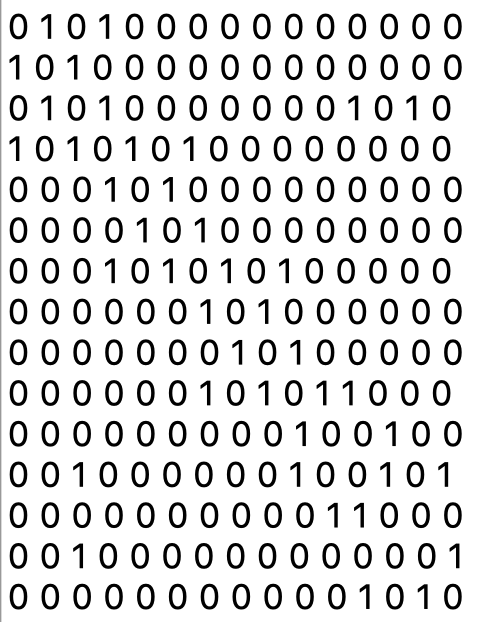
\includegraphics[width = 0.20\linewidth]{figs/h}
  \end{figure}

  其矩阵$G$如上。\\

  \begin{figure}[htbp]
    \centering
    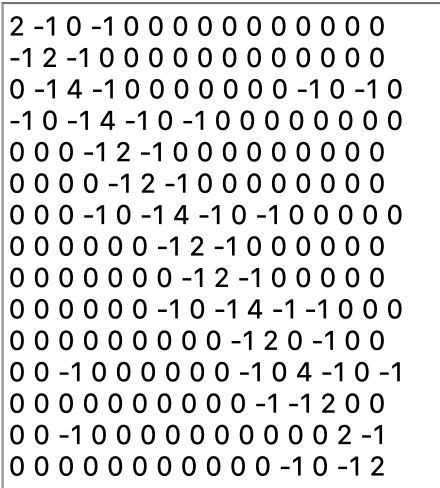
\includegraphics[width = 0.20\linewidth]{figs/i}
  \end{figure}
  其矩阵$C$如上。\\

  经过计算,其共有$3840$个生成树。
\end{solution}
%%%%%%%%%%%%%%%
%%%%%%%%%%%%%%%%%%%%
\beginoptional


%%%%%%%%%%%%%%%%%%%%
\beginot
%%%%%%%%%%%%%%%
%%%%%%%%%%%%%%%
\begin{ot}[Chu–Liu/Edmonds algorithm]
  \begin{itemize}
    \item 	In graph theory, an arborescence is a directed graph in which, for a vertex u called the root and any other vertex $v$, there is exactly one directed path from $u$ to $v$.

    \item In graph theory, Edmonds' algorithm or Chu–Liu/Edmonds' algorithm is an algorithm for finding a spanning arborescence of minimum weight (sometimes called an optimum branching).

  \end{itemize}

  参考资料:\href{https://en.wikipedia.org/wiki/Edmonds%27_algorithm}{https://en.wikipedia.org/wiki/Edmonds\%27\_algorithm}

\end{ot}

% \begin{solution}
% \end{solution}
%%%%%%%%%%%%%%%

\begin{ot}[Minimum bottleneck spanning tree]
  In mathematics, a minimum bottleneck spanning tree (MBST) in an undirected graph is a spanning tree in which the most expensive edge is as cheap as possible.

  参考资料:\href{https://en.wikipedia.org/wiki/Minimum_bottleneck_spanning_tree}{https://en.wikipedia.org/wiki/Minimum\_bottleneck\_spanning\_tree}
\end{ot}

% \begin{solution}
% \end{solution}
%%%%%%%%%%%%%%%




% \vspace{0.50cm}
%%%%%%%%%%%%%%%
% \begin{ot}[]
% 
%   \noindent 参考资料:
%   \begin{itemize}
%     \item 
%   \end{itemize}
% \end{ot}

% \begin{solution}
% \end{solution}
%%%%%%%%%%%%%%%

%%%%%%%%%%%%%%%%%%%%
% 如果没有需要订正的题目,可以把这部分删掉

% \begincorrection
%%%%%%%%%%%%%%%%%%%%

%%%%%%%%%%%%%%%%%%%%
% 如果没有反馈,可以把这部分删掉
\beginfb

% 你可以写
% ~\footnote{优先推荐 \href{problemoverflow.top}{ProblemOverflow}}:
% \begin{itemize}
%   \item 对课程及教师的建议与意见
%   \item 教材中不理解的内容
%   \item 希望深入了解的内容
%   \item $\cdots$
% \end{itemize}
%%%%%%%%%%%%%%%%%%%%
% \bibliography{2-5-solving-recurrence}
% \bibliographystyle{plainnat}
%%%%%%%%%%%%%%%%%%%%
\end{document}